% Chapter 1

\chapter{Introduction}

\label{introduction}
The following thesis will expose and explain the design, techniques, and development done and achieved to create a Music Genre Classifier based on its deep features.

The thesis explores the connections that may appear between musical pieces when combined using Deep Learning approaches as Artificial Neural Networks.

This project consists of the following stages:

\begin{itemize}
    \item Prepare the development environment and programming stack.
    \item Preprocessing of the provided data for the ease of use.
    \item Building of the appropriate dataset selecting the desired features and contents.
    \item Create the Artificial Neural Network model and the needed tools associated with it.
    \item Train the proposed model
    \item Evaluate the results and re-iterate the process to improve model accuracy.
\end{itemize}
  
The next sections will deeply explain and expose the decisions taken during the process of meeting the proposed requirements.
\newpage
%----------------------------------------------------------------------------------------

\section{Motives}
The motives behind this thesis roots in combining music with Artificial Intelligence techniques.

Artificial Neural Networks are a relatively new tool in the Machine Learning field that allows prototyping and creating capable models of virtually any learning task a human can reproduce.

Music genre classification has always been an important topic for the people who enjoy it. Labeling songs according to some formal and style features allow humans to enjoy a certain range of music compositions that better matches their preferences. The music classification also opens the possibility of creating recommender systems that provide the user with a variety of new compositions that the user might enjoy based on the proximity of the bunches several categories fall into. On top of that labeling, music provides a way to connect individual pieces with feelings and moods so the user can experience those mentioned just by listening to the appropriate song that may arise that feeling in them.

Music is a really powerful tool and a great expression of art that brings society together that must not be left unattended.

Combining these two distinctive facets is a considerable feat not to be interesting enough to left without exploring.

The author in this thesis is deeply interested in finding these connections previously mentioned and with the appropriate knowledge in both fields described to achieve the established goals.
\newpage
%----------------------------------------------------------------------------------------

\section{Objectives}
This thesis aims to create a classifier that labels songs with one or more genres looking for the best accuracy when facing new pieces. The project finds to create a model capable of properly labeling songs using its deep features rather than the song itself and establish a mathematical connection between the compositions and the genre or genres it may contain.

Artificial Neural Networks are a trendy topic that has been using for classification duties quite recently with still several aspects yet to be untwined and discovered

This project may serve itself as a complete activity with the achieved conclusions or as a preliminary base for future projects using the outcome obtained in the mentioned thesis.

\newpage
%----------------------------------------------------------------------------------------
\section{Legal Framework}
Defining ethical limits and regulatory laws for Artificial Intelligence applications is still a pending task.
There are several factors to weighted in and aspects that may clash with the human natural ethics.
The oportunity of creating sentient machines raises a host of ethical issues. 
These questions relate both to ensuring that such machines do not harm humans or any other beings, and to the moral status of the machines themselves \cite{}. 


Even without a legal framework, the concerning of ethical issues is an important factor when developing autonomous applications.
When the system fails the responsability shall be defined and clearly exposed. 
To bring an example Tesla is facing a legal lawsuit due to the recent fatal crash of one his autopiloted cars \cite{tesla}.

In addition to the moral dilemma the AI machines present a data regulation should be adressed too.
Tupically, these applications heavily rely on huge amounts of data used for training and testing and all the information included must comply with the vigent law.
In Spain the General Data Protection Regulation (GPDR) establish the customer rights about data and privacy among others against thrid party entities.

Regarding the intelectual property, the spanish law grants acknowledgment, economic retribution and other benefits to its authors or sole author

Any piece of Open Source software developep shall require a License.
Generally, any Open Source software is software that can be freely accessed, used, changed, and shared (in modified or unmodified form) by anyone. 
Open source software is made by many people, and distributed under licenses that comply with the Open Source Definition \cite{opensource} \cite{opensourcedef}.


\newpage

\section{Socio-economic environment}
\subsection{Budget}

This thesis is meant to be completed within 4 months and 12 ECTS worth. 
According to the 'European Credit Transfer and Accumulation System \cite{EuropeanCommission2009}', 
a credit constitutes about 25 to 30 student hours which means 12 ECTS * 30 hours = 360 plus a 10\% of possible overload, would sum up roughly 400 hours of student time.

Including 1h weekly meetings with the supervisor during 19 weeks, this adds up to 19 hours plus a 6 hours margin gives a total of 25 hours.

\begin{table}[h!]
    \centering
    \begin{tabular}{l l l l} 
        \hline
        Labour & Cost per hour & Total hours & Total \\ [0.5ex] 
        \hline
        Student & 12 & 400 & 4800 \\ 
        Supervisor & 20 & 25 & 500 \\
        \hline
        & & Sum & 5300 \\
        \hline
    \end{tabular}
    \caption{Human Resoures summary}
    \label{table:Human Resoures summary}
\end{table}

Given all the software used is open-source there are no licensing-related additional costs and all the included costs are equipment related.

The assets include 2 computers, 1 laptop Xiami Mi Air used for prototyping and quickly sketching and one custom-built desktop with an i5-9400F CPU, 16Gb of RAM and an NVIDIA GTX 1050 TI GPU 
To calculate its value a simple depreciation formula is used:
$$Usage *  (Asset Cost - Residual Value) / Useful Life Of The Asset$$
Using the formula the costs of the assets are:
\begin{table}[h!]
    \centering
    \begin{tabular}{l l l l l l} 
        \hline
        Device & Asset Cost & Residual Value & Useful life of the asset (years) & Usage & Total \\ [0.5ex] 
        \hline
        Laptop & 900 & 200 &  4 & 1 & 175 \\ 
        Desktop & 1300 & 400 & 6 & 1 & 150 \\
        \hline
        & & & & Sum & 325 \\
        \hline
    \end{tabular}
    \caption{Assets summary}
    \label{table:2}
\end{table}

The indirect costs, including gas, electricity, bills, internet, water and other related matters are assumed as 20\% of the total amount of the assets costs.

\begin{table}[h!]
    \centering
    \begin{tabular}{l l} 
        \hline
        Expenses & Value \\
        \hline
        Human Labour & 5300 \\ 
        Assets & 325 \\
	    Indirect costs & 65 \\
        \hline
        Sum & 5690 \\
        \hline
    \end{tabular}
    \caption{Budget Summary}
    \label{table:Budget Summary}
\end{table}
\newpage

\subsection{Impact}
% TODO
\newpage

\section{Artificial Neural Networks}
\begin{figure}[th]
    \centering
    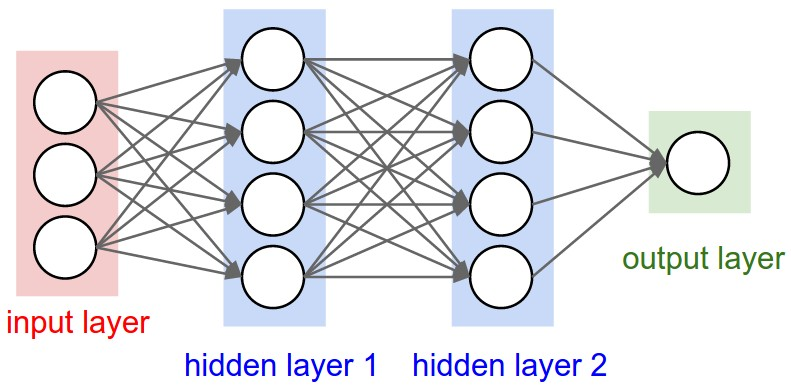
\includegraphics[width=1.0\textwidth]{Figures/NeuralNet}
    \decoRule
    \caption[Simple MLP architecture]{Simple MLP architecture (Image credit \cite{cs231n})}
    \label{fig:mlp}
\end{figure}

The mathematical model of a single neuron share some resemblance with the biological one.
A biological neuron receives input from its dendrites as an electrical signal that is outputted through the axon to the next neuron in the chain.
The mathematical model uses this baseline and takes the input $x_i$ for each of the dendrites and multiplies it by the corresponding weight $w_i$,
depending on the weight of the strength of the neuron will be higher. 

\begin{figure}[th]
    \centering
    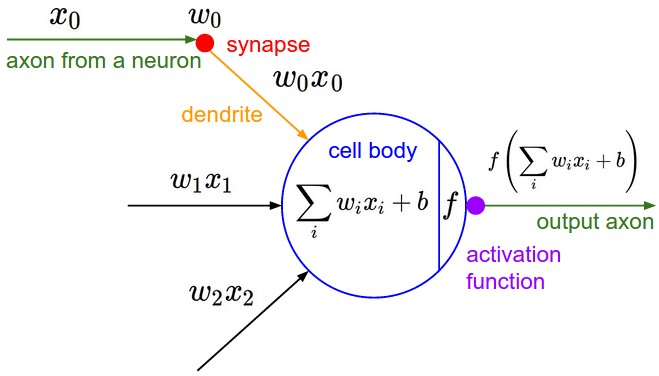
\includegraphics[width=1.0\textwidth]{Figures/Neuron}
    \decoRule
    \caption[Neuron Mathematical model]{Neuron Mathematical model (Image credit \cite{cs231n})}
    \label{fig:neuron}
\end{figure}

If we compute this for every input $x_i$ and every weight $w_i$ we get the vector dot multiplication

$$ \sum_{i=1} x_i w_i  $$ 

Adding a bias factor $b$:

$$ \sum_{i=1} x_i w_i  + b$$ 

And using an activation function $f$:

$$ f(\sum_{i=1} x_i w_i + b)  $$ 

The activation function will apply a mathematical operation at element level thresholding the output

\begin{figure}
    \centering
    \begin{subfigure}{.5\textwidth}
        \centering
        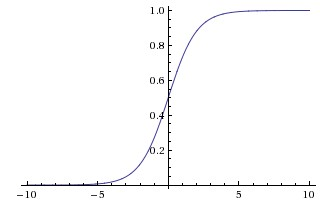
\includegraphics[width=.4\linewidth]{Figures/sigmoid}
        \caption{sigmoid activation function}
        \label{fig:sub1}
    \end{subfigure}%
    \begin{subfigure}{.5\textwidth}
        \centering
        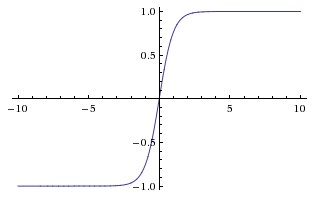
\includegraphics[width=.4\linewidth]{Figures/tanh}
        \caption{tanh activation function}
        \label{fig:sub2}
    \end{subfigure}
    \caption{Activation functions examples (Image credit \cite{cs231n})}
    \label{fig:activations}
\end{figure}



We can generalize this model for any number of neurons $n$:

$$
W=\left[
\begin{array}{ccc}
   w_{11} & \cdots & w_{1i} \\
   \vdots & \ddots & \vdots \\
   w_{n1} & \cdots & w_{ni}
\end{array}
\right]
$$

And for any number of examples $m$:

$$
X=\left[
\begin{array}{ccc}
   x_{11} & \cdots & x_{1m} \\
   \vdots & \ddots & \vdots \\
   x_{i1} & \cdots & x_{im}
\end{array}
\right]
$$

Therefore the complete output of a MLP is
$$ A = f(WX + b) $$


In case we stack several layers the output $A$ of this layer becomes the input of the next one

$$ A_j = f_j(W_jA_{j-1} + b_j) $$

If we want to obtain the output matrix $\hat{Y}$ we need to check the output of the last layer $l$:

$$ \hat{Y} = A_l $$

Once the output $\hat{Y}$ is obtained we can check the error against the real output $Y$:

$$ E = || \hat{Y} - Y || $$

During the training phase, the Network will try to adjust the weights matrixes $W_j$ minimizing the error $E$.
To do so the Gradient Descent is used to find the global minima of the loss function:

\begin{figure}[th]
    \centering
    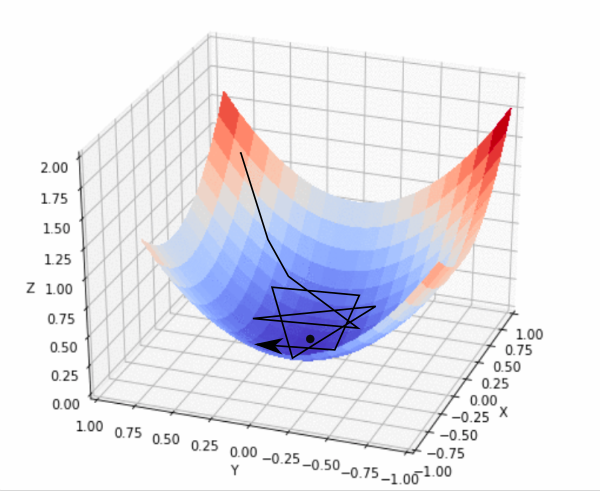
\includegraphics[width=1.0\textwidth]{Figures/GDescent.png}
    \decoRule
    \caption[Gradient Descent]{Gradient Descent (Image credit \cite{mathann})}
    \label{fig:Gradient Descent}
\end{figure}

To calculate the Gradient Descent complex partial derivatives are used that will not be discussed in this paper as it is out of the scope of the mentioned \cite{Suykens1996}.